\newcommand{\HeaderLineSpace}{-0.25cm}

\newcommand{\UniTextRO}{UNIVERSITATEA POLITEHNICA DIN BUCUREȘTI \\[\HeaderLineSpace]
FACULTATEA DE AUTOMATICĂ ȘI CALCULATOARE \\[\HeaderLineSpace]
DEPARTAMENTUL DE CALCULATOARE\\}
\newcommand{\DiplomaRO}{PROIECT DE DIPLOMĂ}
\newcommand{\AdvisorRO}{Coordonator științific:}
\newcommand{\BucRO}{BUCUREȘTI}

\newcommand{\UniTextEN}{UNIVERSITY POLITEHNICA OF BUCHAREST \\[\HeaderLineSpace]
FACULTY OF AUTOMATIC CONTROL AND COMPUTERS \\[\HeaderLineSpace]
COMPUTER SCIENCE AND ENGINEERING DEPARTMENT\\}
\newcommand{\DiplomaEN}{DIPLOMA PROJECT}
\newcommand{\AdvisorEN}{Thesis advisor:}
\newcommand{\BucEN}{BUCHAREST}

\newcommand{\frontPage}[6]{
\begin{titlepage}
\begin{center}
{\Large #1}  % header (university, faculty, department)
\vspace{50pt}
\begin{tabular}{p{5cm}p{5cm}}
\includegraphics[scale=0.8]{img/logos/upb-logo.jpg} &
	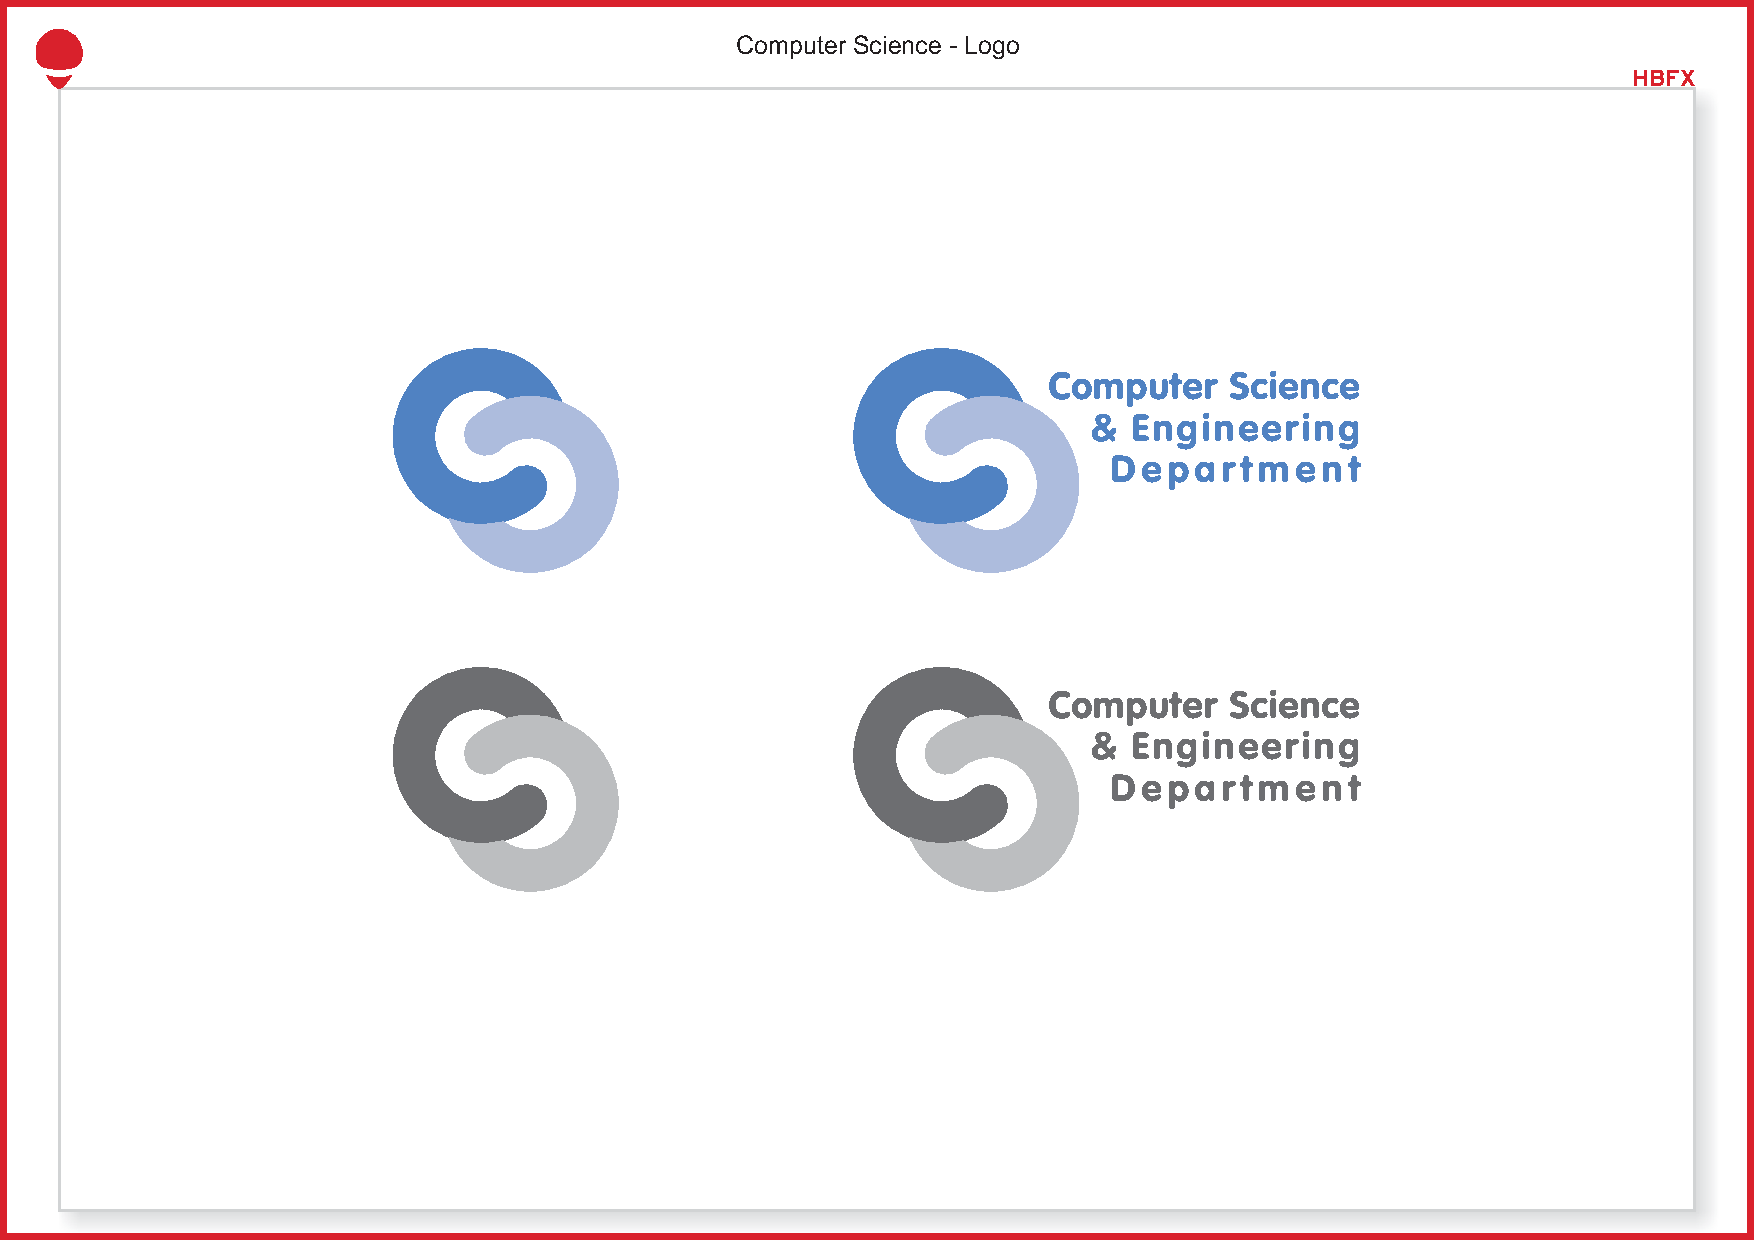
\includegraphics[scale=0.5,trim={14cm 11cm 6cm 5cm},clip=true]{img/logos/cs-logo.pdf}
\end{tabular}

\vspace{105pt}
{\Huge #2}\\                           % diploma project text
\vspace{40pt}
{\Large #3}\\ \vspace{0pt}  % project title
% {\Large #4}\\                          % project subtitle
\vspace{40pt}
{\LARGE \Name}\\                   % student name
\end{center}
\vspace{60pt}
\begin{tabular*}{\textwidth}{@{\extracolsep{\fill}}p{6cm}r}
&{\large\textbf{#4}}\vspace{10pt}\\      % scientific advisor
&{\large \AdvisorA}\vspace{10pt}\\                       % advisor 1 name
&{\large \AdvisorB}                         % advisor 2 name
\end{tabular*}
\vspace{20pt}
\begin{center}
{\large\textbf{#5}}\\                                % bucharest
\vspace{0pt}
{\normalsize \Year}
\end{center}
\end{titlepage}
}

\newcommand{\frontPageEN}{\frontPage{\UniTextEN}{\DiplomaEN}{\ProjectTitleEN}{\AdvisorEN}{\BucEN}}
\newcommand{\frontPageRO}{\frontPage{\UniTextRO}{\DiplomaRO}{\ProjectTitleRO}{\AdvisorRO}{\BucRO}}

\linespread{1.15}
\setlength\parindent{0pt}
\setlength\parskip{.28cm}

%% Abstract macro
\newcommand{\AbstractPage}{
\begin{titlepage}
\textbf{\large ABSTRACT}\par
\AbstractEN \vfill
\textbf{\large SINOPSIS}\par
\AbstractRO\par\vfill
\end{titlepage}
}

%% Thank you macro
% \newcommand{\ThanksPage}{
% \begin{titlepage}
% {\noindent \large\textbf{MULȚUMIRI}}\\
% \Thanks
% \end{titlepage}
% }

%%%%%%%%%%%%%%%%%%%%%%%%%%%%%%%%%%%%%%%%%%%%%%%%%%
%%
%%          End of template definitions
%%
%%%%%%%%%%%%%%%%%%%%%%%%%%%%%%%%%%%%%%%%%%%%%%%%%%

%%
%%   Campurile de mai jos trebuie modificate de autor. Modificati doar continutul, nu si numele fiecarei definitii
%%
\newcommand{\ProjectTitleEN}{Automatic Tire-markings Detection \& Recognition}
\newcommand{\ProjectTitleRO}{Detectarea și Recunoașterea Automată a Marcajelor de pe Cauciucuri}
\newcommand{\Name}{Robert-Mihai Lică}
\newcommand{\AdvisorA}{
    Conf. dr. ing. Iuliu Vasilescu
}
\newcommand{\AdvisorB}{
    Conf. dr. ing. Daniel Rosner
}

\newcommand{\Year}{2022}

% Setări document
\title{Proiect de diplomă}
\author{\Name}
\date{\Year}

%%
%%   Campurile aferente rezumatului
%%
\newcommand{\AbstractEN}{This work shall provide an image processing pipeline for automatic detection and recognition of tire-markings from images. Because tires can be one of the most expensive consumables of a truck, they are of interest to fleet managers who want to monitor their placement, parameters and possible illegal swap. My solution shall provide an easy way to extract from an image the serial code and/or certification number in order to aid an individual to almost uniquely identify a tire. The system can identify a wheel in an image and unwraps it. Then, it detects the text regions on the tire by using a band-pass filter on the frequency domain of the image, and lastly Microsoft Cognitive Services' OCR is employed to perform the character recognition.}

\newcommand{\AbstractRO}{Această lucreare o să ofere o bandă de procesare a imaginilor pentru detectarea automată și recunoașterea marcajelor de pe marginea unui cauciuc. Deoarece cauciucurile pot fi unul dintre cele mai scumpe consumabile ale unui tir, este în interesul managerilor de flote să monitorizeze utilizarea cauciucurilor, parametrii lor și eventuale schimbări ilegale. Soluția mea va oferi o metodă ușoară de a extrage din imagini codul de serie și/sau numărul certificării pentru a identifica aproape unic un cauciuc. Sistemul poate să identifice o roată într-o imagine și să o desfășoare. Apoi, aplică un filtru bandă pe domeniul de frecvență a imaginii și OCR-ul de la "Microsoft Cognitive Services" este utilizat pentru a efectua recunoașterea caracterelor.}

%%
%%   Campurile aferente paginii de multumiri
%%
% \newcommand{\Thanks}{(opțional) Aici puteți introduce o secțiunea specială de mulțumiri / acknowledgments. }
